\documentclass{report}
\usepackage[utf8]{inputenc}
\usepackage{graphicx}
\usepackage{multirow}
\usepackage{caption}
\usepackage{subcaption}
\usepackage{amsfonts,amssymb,amsmath}
\usepackage{multicol}
\usepackage{listings}
\usepackage{enumitem}
\lstset{
  basicstyle=\ttfamily,
  mathescape
}
\usepackage[utf8]{inputenc}
\usepackage[spanish]{babel}
\usepackage{lscape}
\usepackage[left=1.5cm,right=1.5cm,top=2cm,bottom=2cm]{geometry}

\begin{document}

\begin{center}
    
    \begin{tabular}{l c r}
    
\includegraphics[scale=0.15]{Imagenes/IPN.jpeg}
    & 
        \bf\fontsize{22}{0}{\selectfont{Instituto Polit\'ecnico Nacional}}

    
    & 
\includegraphics[scale=0.08]{Imagenes/escom.png} \\
     
    & \bf\fontsize{22}{0}{\selectfont{ Escuela Superior de C\'omputo}} &  \\
    \end{tabular}

	
	\vspace*{2\baselineskip}
	
	{
		\bf\fontsize{12}{0}{\selectfont{An\'alisis de Algoritmos, Sem: 2021-1, 3CV1, Pr\'actica 6, 14/12/20}}
	}
			
	\vspace*{2\baselineskip}
			 
	{
		\fontsize{23}{0}{\selectfont{Práctica 6: Algoritmos greedy, Programación Dinámica}}
	}
	
	\vspace*{2\baselineskip}
	
	{
		\bf\fontsize{12}{0}{\selectfont{Valle Mart\'inez Luis Eduardo, Rivero Ronquillo Omar Imanol}}
	}
	
	\vspace*{1\baselineskip}
	
	{
		\fontsize{12}{0}{\textit{lvalle212@gmail.com, imanol.rivero7@gmail.com}}
	}
	
	\vspace*{2\baselineskip}

    {
	    \fontsize{12}{0}\selectfont{
	    \textbf{Resumen:} En el actual documento se presenta el análisis de algoritmos que operan bajo la estrategia de búsqueda voraz o también llamados \textbf{Greedy} y algoritmos que operan mediante programación dinámica}
	    
	    \fontsize{12}{0}\selectfont{
	    \textbf{Palabras Clave:} Programación Dinámica, Fibonacci, Mochila 0-1, Java }
	
	}
\end{center}

\chapter*{Introducción} 
    Para la creación de un algoritmo existen distintos métodos y enfoques ahora ya bastante bien conocidos y estudiados, tales como los secuenciales, los recursivos, los Greedy o voraces, etc. Y además de los anteriores aquellos que nos encontramos analizando en esta práctica, los que implementan la programación dinámica mediante el uso de memoización, en la mayoria de los casos. Sin embargo, para hacer uso de estos enfoques nuestro problema deberá cumplir con ciertas condiciones, que más adelante serán mencionadas.

Como podemos ver, se cuenta con una amplia gama de técnicas y muy probablemente no sea tan sencillo escoger entre ellas, pero finalmente es tarea de la ingeniería conocer todos estas técnicas y enfoques para finalmente elegir cúal es el que hace mejor se adapta a la problematica que se busca resolver.

Los algoritmos que se analizan y prueban en este documento son algoritmos clásicos bien estudiados por todos aquellos profesionales pertenecientes a las ciencias de la computación, pero esta reputación de clásicos, no se debe solamente a que ejemplifican perfectamente el uso de los métodos con las que son implementadas, pero por que son simplemente útiles para la resolución de problemáticas con las que cotidianamente lidian, tanto profesionales como no expertos en el área donde surge la necesidad de encontrar solución a una situación.

Siendo una de las sucesiones de números más fascinantes que encontramos directamente describiendo fenómenos de la naturaleza con Fibonacci. O el amplio abanico de problemas en los que puede implementarse, mediante variaciones del problema original, la Mochila entera para encontrar la solución a problemas específicos de un área.

\chapter*{Conceptos B\'asicos}
   \section*{Divide y vencerás}
    El nacimiento de esta frase se remonta al gran Julio César, prestigioso militar y político romano nacido en los años 100 a.C., teniendo su origen en el hecho de que los romanos al conquistar un territorio, se abstenían de oprimir a los vencidos, evitando rebeliones y la formación de un frente común. Para evitar esto, además los romanos firmaban contratos con cada pueblo de manera individual, otorgando derechos distintos y de número irregular a cada uno, provocando envidias entre los mismos pueblos, y por consiguiente imposibilitando la unión.\\
    
    Con el pasar del tiempo, se convirtió en un refrán popular que implica resolver un problema difícil, dividíendolo en partes más simples tantas veces como sea necesario, hasta que la solución de las partes sea obvia, de esta forma la solución del problema principal se construye con las soluciones encontradas.\\
    
    De esta forma llegó hasta las ciencias de la computación, convirtiéndose en uno de los paradigmas más importantes en el diseño algorítmico. Esta basado en la resolución recursiva de un problema que se divide un subproblemas del mismo tipo hasta que resulten lo suficientemente sencillos para realizar de forma directa. El resultado final entonces, se conforma de la combinación  de los resultados de los subproblemas, dando una solución final al problema general.\\
    
    De esta técnica se tienen algoritmos muy eficientes para la resolución de cualquier tipo de problema, ejemplos basados en esta técnica se tiene:\\
    \begin{itemize}
        \item Algoritmo de Ordenamiento: QuickSort, MergeSort
        \item Multiplicar números grandes: Karatsuba
        \item Análisis sintáctico: análisis sintáctico top-down
        \item Transformada discreta de Fourier
    \end{itemize}
    
\section*{Algoritmos de ordenamiento}
    Los algoritmos de ordenamiento son algoritmos que colocan los elementos de un array, lista o vector, en una secuencia específica descrita por una relación de orden.\\
    
    Los órdenes más comunes son el numérico y lexicográfico, siendo el último una relación de orden definida sobre el producto cartesiano de conjuntos ordenados. Es principalmente concido por la aplicación a cadenas de caracteres en diccionarios, guias telefónicas, etc.\\
    
    La salida de estos algoritmos deben de satisfacer 2 condiciones:
    \begin{enumerate}
        \item La salida debe de encontrarse en orden no-decreciente
        \item La salida es una permutación o re-ordenamiento de la entrada
    \end{enumerate}
    
    Hay métodos muy simples de implementar que son útiles en los casos en dónde el número de elementos a ordenar no es muy grande. Pero por otro lado hay métodos sofisticados, más difíciles de implementar pero que son más eficientes en cuestión de tiempo de ejecución.
    
    Los métodos sencillos por lo general requieren de aproximadamente n x n pasos para ordenar n elementos.
    
    Los métodos simples con complejidad cuadrática son:
    \begin{itemize}
        \item Insertion Sort
        \item Selection Sort
        \item Bubble Sort
        \item Shell Sort(extensión más veloz del bubble sort)
    \end{itemize}
    
    Los métodos más complejos acortan el tiempo de ejecución y por lo tanto son más eficiente:
    \begin{itemize}
        \item Quick Sort
        \item Merge Sort
        \item Heap Sort
        \item Radix
        \item Address-calculation Sort
    \end{itemize}
    
    Existen diferentes maneras de clasificar los algoritmos de ordenamiento:
    
    \textbf{Clasificación según el lugar donde se realiza la ordenación}\\
    \begin{itemize}
        \item Ordenamiento interno: Se realiza el ordenamiento enteramente en la memoria primaria del ordenador
        \item Ordenamiento externo: Aquellos que involucran discos auxiliares para guardar resultados intermedios
    \end{itemize}
    
    \textbf{Clasificación por el tiempo que tardan en la ordenación}\\
    \begin{itemize}
        \item Ordenación natural: Tarda lo mínimo posible con la entrada ordenada
        \item Ordenación no natural: Tarda lo mínimo posible cuando la entrada esta inversamente ordenada 
    \end{itemize}
    
    \textbf{Por estabilidad}\\
    En un ordenamiento estable se mantiene el orden relativo que tenian originalmente los elementos con claves iguales. Esto es, con un algoritmo estable habrá 2 registros R y S con la misma clave y con R apareciendo antes que S en la lista original.\\
    
    En elementos que son indistiguibles entre si, la estabilidad no es un problema, tal y como sucede con los números enteros, pero en general se puede decir que se despecia la estabilidad cuando el elemento entero es la clave.\\
    
\section*{Merge Sort}
    Merge Sort es un algoritmo desarrollado con la técnica de divide y vencerás, creado por Jhon Von Newmann en 1945. De propósito general, es un algoritmo que produce un ordenamiento estable con complejidad O(nlogn). Utiliza memoria auxiliar con complejidad O(n), dado por el algoritmo \textit{Merge}.\\
    
    La familia de algoritmos \textit{Merge}, toman una multiple lista ordenada como entrada y produce una lista única ordenada como salida, conteniendo todos los elementos de la lista de entrada. Estos algoritmos son utilizados como subrutinas para varios algoritmos de ordenamiento, siendo el más famoso precisamente \textit{Merge Sort}.\\
    
    \textit{Merge Sort} inicia con la entrada de un arreglo, este divide el arreglo de entrada en 2 mitades, se llama a si mismo para las 2 mitades y después mezcla las mitades con ayuda del algoritmo \textit{Merge}.\\
    
    Gráficamente la operación del algoritmo se muestra en la siguiente figura \ref{OperacionMergeSort}:
    \begin{figure}[h!]
        \centering
        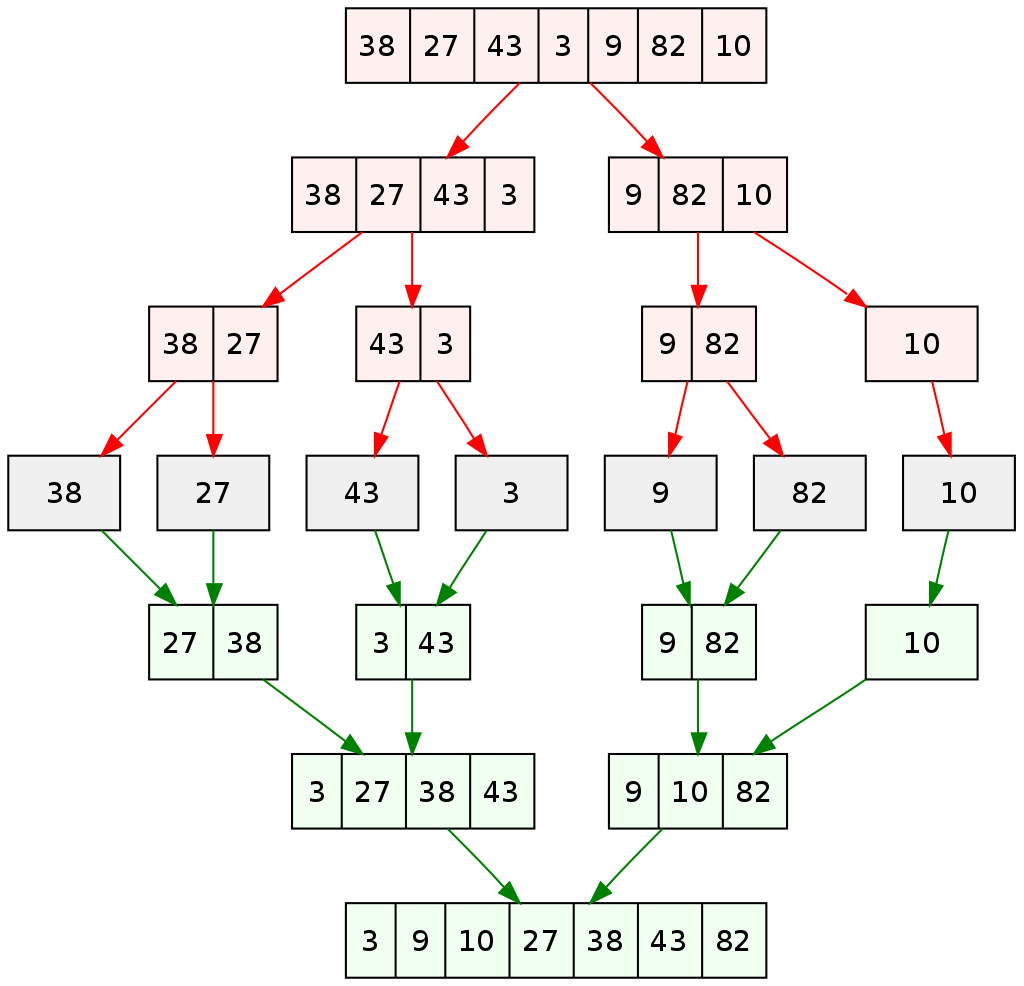
\includegraphics[width=10cm]{OperacionMergeSort.png}
        \caption{Ordenamiento de un arreglo de 7 valores enteros utilizando el algoritmo \textit{MergeSort}}
        \label{OperacionMergeSort}
    \end{figure}
    
\section*{Quick Sort}
    Quick Sort es un algoritmo basado en la técnica divide y vencerás creado por el científico británico C. A. R. Hoare, quién también es conocido como Tony Hoare, en el año de 1960.\\
    
    Es el algoritmo más ampliamente utilizado en el mundo para el ordenamiento numérico, también es considerado el algoritmo más eficiente y veloz de los métodos de ordenación interna.
    
    La complejidad del algoritmo para su caso promedio es O(nlogn), pero en su peor caso tendrá la complejidad O($n^2$), dandose este caso cuando el pivote queda en alguno de los extremos.
    
    El funcionamiento del algoritmo se describe en 4 pasos:\\
    \begin{enumerate}
        \item Se elige un elemento de la lista a ordenar, se le llamará pivote
        \item Se reacomodan los elementos de la lista según el valor de pivote, de manera que los elementos antes de este son siempre menores, y los que están después serán siempre mayores. Después de este ordenamiento parcial, el pivote ya se encuentra colocado en el lugar exacto que debe ocupar en la lista final.
        \item La lista se separa en 2 sublistas, una formada por los elementos a la izquierda del pivote, y otra por los elementos a su derecha.
        \item Se repite el proceso de forma recursiva para todas las sublistas mientras estas contengan más de un elemento. Al terminar este proceso todos los elemento se encuentran ordenados.
    \end{enumerate}
    
    En este algoritmo la elección del pivote es muy importante, pues dependiendo de la elección, el algoritmo puede ser más o menos eficiente. Si bien tomar un elemento cualquiera como pivote no requiere de cálculo alguno, la elección a ciegas puede provocar para ciertas entradas una complejidad de O($n^2$).\\
    
    Una alternativa para subsanar este problema es conocer de antemano el elemento central para utilizar como pivote, esta operación puede realizarse en O(n) y asegura hasta para el peor de los casos que el algoritmo sea O(nlogn), sin embargo este cálculo adicional rebaja la eficiencia en el caso promedio.\\
    
    Otra opción es tomar tres elementos de la lista, comúnmente se escoge el primero, medio y último elemento del arreglo, se comparan y el valor medio es escogido como el pivote.

\chapter*{Experimentación y Resultados}
    \section*{Algoritmo de Fibonacci}
        Debido a la naturaleza de la sucesión de Fibonacci contamos con diferentes formas para expresar un algoritmo para obtener los elementos de la sucesión. A continuación realizaremos una comparación del algoritmo en su presentación usual, es decir, el que calcula el elemento mediante recursividad, y mediante programación dinamica, en sus enfoques Top-Down y Bottom-Up.

\subsection*{Análisis a posteriori}
    Para la realización de nuestra gráfica, se realizó un conteo del número de operaciones realizadas por cada algoritmo para cada entrada n, siendo n el enésimo elemento de la sucesión de Fiboncci. A continuación en las figuras \ref{TablaFiboTop}, \ref{TablaFiboBottom} y \ref{TablaFiboRec}, se presentan los pares ordenados considerados en la gráfica.
    
    \begin{figure}[h!]
        \centering
        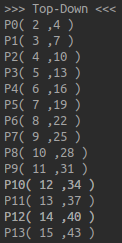
\includegraphics[width=5cm]{Fibonacci/tab-fibo-top.png}
        \caption{Pares ordenados obtenidos para el algoritmo de Fibonacci con programación dinámica utilizando el enfoque Top-Down.}
        \label{TablaFiboTop}
    \end{figure}
    \newpage
    \begin{figure}[h!]
        \centering
        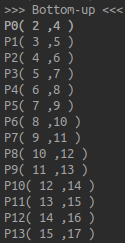
\includegraphics[width=5cm]{Fibonacci/tab-fibo-botttom.png}
        \caption{Pares ordenados obtenidos para el algoritmo de Fibonacci con programación dinámica utilizando el enfoque Bottom-Up.}
        \label{TablaFiboBottom}
    \end{figure}
    
    \begin{figure}[h!]
        \centering
        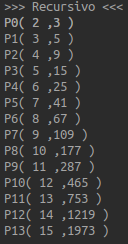
\includegraphics[width=5cm]{Fibonacci/tab-fibo-rec.png}
        \caption{Pares ordenados obtenidos para el algoritmo de Fibonacci en su presentación usual a través de recursividad.}
        \label{TablaFiboRec}
    \end{figure}
    
    \newpage

    Fueron considerados únicamente 14 puntos para cada algoritmo para que siguiera siendo posible apreciar las pequeñas diferencias que presentan los dos enfoques de programación dinámica. Cada uno de los puntos, tiene como abscisa a n, siendo el enésimo elemento de la sucesión de Fibonacci y como ordenadas al número de operaciones realizadas por el algoritmo. Finalmente, observamos en la figura \ref{GraficaFibonacci} la gráfica que representa los pares de puntos obtenidos.
    
    \begin{figure}[h!]
        \centering
        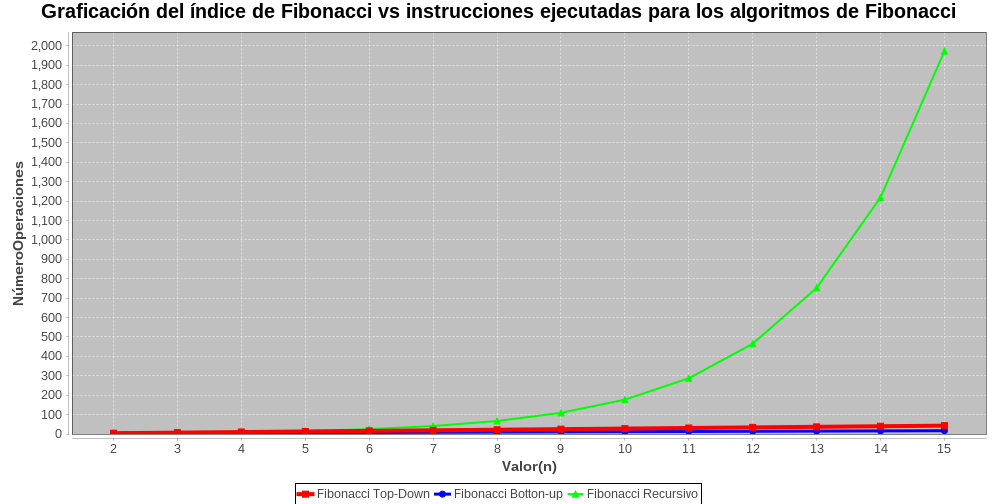
\includegraphics[width=18cm]{Fibonacci/fibo-din-graph.png}
        \caption{Grafica obtenida de la comparación de los algoritmos para el cálculo del enésimo elemento de la sucesión de Fibonacci mediante el conteo del número de operaciones realizadas en cada caso.}
        \label{GraficaFibonacci}
    \end{figure}
    \newpage
    A continuación, en la figuras \ref{GraficaDesmosFiboDinamico} y \ref{GraficaDesmosFiboRecu}, se muestra la comparación de los puntos encontrados experimentalmente para estos algoritmos para el cálculo del enésimo elemento de la sucesión de Fibonacci mediante programación dinámica y con recursividad simple, contra nuestra propuesta de ecuación que describe la complejidad temporal de los mismos.
    
    \begin{figure}[h!]
        \centering
        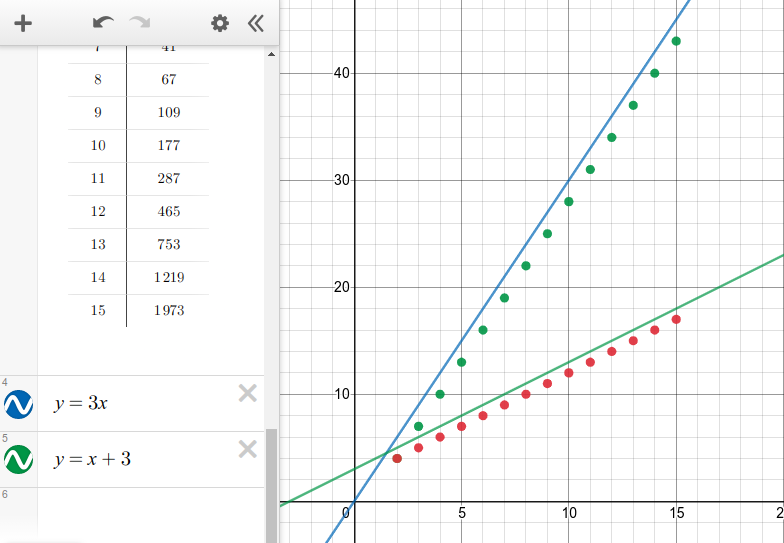
\includegraphics[width=18cm]{Fibonacci/fibo-graph-desm1.png}
        \caption{Representación gráfica de la complejidad temporal de los algoritmos de Fibonacci usando programación dinámica comparada con nuestras propuestas de ecuaciones que los acotan}
        \label{GraficaDesmosFiboDinamico}
    \end{figure}
    
    En la figura \ref{GraficaDesmosFiboDinamico}, los puntos de color verde representan los pares ordenados obtenidos mediante el enfoque Top-Down, mientras que los de color rojo representan los pares ordenados obtenidos con el enfoque Bottom-Up. La recta $y=3x$ es nuestra propuesta de ecuación que acota la complejidad temporal para el enfoque Top-Down, y la recta $y=x+3$ es la propuesta de ecuación que acota la complejidad temporal para el enfoque Bottom-Up. Es particularmente interesante observar que aunque los dos enfoques comparten una complejidad lineal dada por $\Theta(n)$, parece por los resultados experimentales que el enfoque Bottom-Up es más eficiente.
    
    \newpage
    
    \begin{figure}[h!]
        \centering
        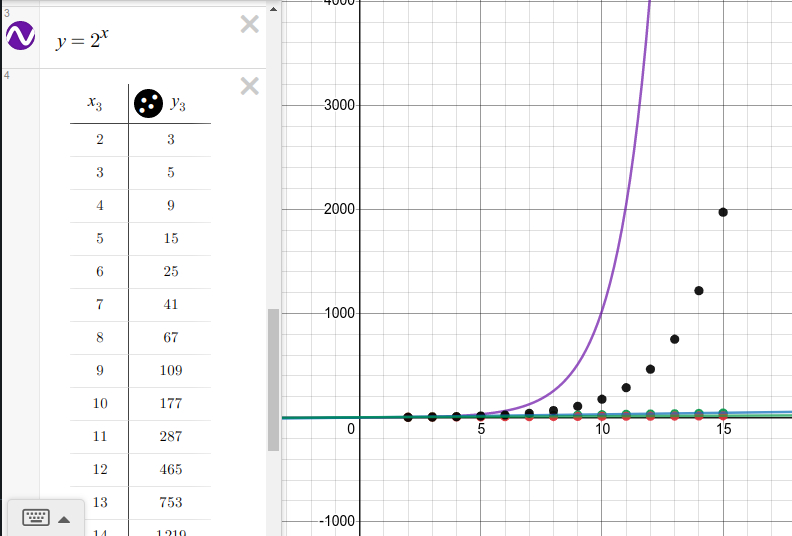
\includegraphics[width=18cm]{Fibonacci/graph-fibo-desm2.png}
        \caption{Representación gráfica de la complejidad temporal del algoritmo de Fibonacci usando su presentación usual de recursividad simple comparada con nuestra propuesta de ecuación que la acota.}
        \label{GraficaDesmosFiboRecu}
    \end{figure}
    
    En la figura \ref{GraficaDesmosFiboRecu}, los puntos en color negro representan los pares ordenados obtenidos por el algoritmo de Fibonacci en su presentación usual. La función $y=2^{x}$ es nuestra propuesta de ecuación que acota la complejidad temporal del algoritmo. Por lo tanto la complejidad temporal esta dada por $\Theta(\phi^{n})$.
    
    Como podemos observar, hay una diferencia abismal entre la cantidad de operaciones realizadas por el algoritmo usando recursividad simple comparado con aquellos que utilizan la programación dinámica para potenciar la eficiencia del cálculo.

\subsection*{Análisis a priori}
    \subsubsection{Fibonacci en su presentación usual}
    Consideremos el pseudocódigo descrito en la figura \ref{PseudocodigoFiboRec} para este algoritmo.
    \begin{figure}[h!]
        \centering
        \begin{verbatim}
            int fiboRec(n:entero)
                if n==0
                    return 0
                else if n==1
                    return 1
                else
                    return fiboRec(n-1)+fiboRec(n-2)
        \end{verbatim}  
        \caption{Pseudocódigo del algoritmo de Fibonacci en su presentación usual.}
        \label{PseudocodigoFiboRec}
    \end{figure}
    \newpage
    A continuación se describe el análisis de complejidad por bloques.
    
    \begin{equation*}
        \left.
            \begin{aligned}
                \left.
                    \begin{aligned}
                        \text{if n==0}\\
                        \text{return 0}\\
                        \text{else if n==1}\\
                        \text{return 1}\\
                    \end{aligned}
                \right\}
                \quad\Theta(1)
                \\
                \left.
                    \begin{aligned}
                        \text{else}\\
                        \text{return fiboRec(n-1)+fiboRec(n-2)}
                    \end{aligned}
                \right\}
                \quad T(n-1)+T(n-2)
                \\
            \end{aligned}
        \right\}
        \quad T(n)=T(n-1)+T(n-2)
    \end{equation*} 
    
    Finalmete, resolviendo la ecuación de recurrencia $T(n)=T(n-1)+T(n-2)$ por el método de ecuación característica, tenemos que la complejidad temporal del algoritmo de Fibonacci en su presentación usual tiene una complejidad temporal $\mathcal{O}(\phi^{n})$.
    
    \subsubsection*{Fibonacci usando programación dinámica con el enfoque Top-Down}
    Consideremos el pseudocódigo descrito en la figura \ref{PseudocodigoFiboTop} para este algoritmo.
    
    \begin{figure}[h!]
        \centering
        \begin{verbatim}
            int fiboTop(n:entero, fibo:tabla)
                if fibo[n] != -1
                    return fibo[n]
                fibo[n] = fiboTop(n-2) + fiboTop(n-1)
                return fibo[n]
        \end{verbatim}  
        \caption{Pseudocódigo del algoritmo de Fibonacci mediante programación dinámica con enfoque Top-Down}
        \label{PseudocodigoFiboTop}
    \end{figure}
    
    A continuación se describe el análisis de complejidad por bloques.
    
    \begin{equation*}
        \left.
            \begin{aligned}
                \left.
                    \begin{aligned}
                        \text{if fibo[n] != -1}\\
                        \text{return fibo[n]}\\
                    \end{aligned}
                \right\}
                \quad\Theta(1)
                \\
                \left.
                    \begin{aligned}
                        \text{fibo[n] = fiboTop(n-2) + fiboTop(n-1)}
                    \end{aligned}
                \right\}
                \quad\Theta(n)
                \\
                \left.
                    \begin{aligned}
                        \text{return fibo[n]}
                    \end{aligned}
                \right\}
                \quad\Theta(1)
                \\
            \end{aligned}
        \right\}
        \quad\Theta(n)
    \end{equation*} 
    
    Finalmente, se concluye que el algoritmo de la sucesión de Fibonacci usando programación dinámica con el enfoque Top-Down tiene una complejidad temporal lineal dada por $\Theta(n)$.
    
    \subsubsection*{Fibonacci usando programación dinámica con el enfoque Bottom-Up}
    Consideremos el pseudocódigo descrito en la figura \ref{PseudocodigoFiboDown} para este algoritmo.
    
    \begin{figure}[h!]
        \centering
        \begin{verbatim}
            int fiboBottom(n:entero, fibo:tabla)
                if n <= 1
                    return 1
                else
                    fibo[0] = 0
                    fibo[1] = 1
                    for i=2 to i<=n do
                        fibo[i]=fibo[i-1]+fibo[i-2]
                return fibo[n]
        \end{verbatim}  
        \caption{Pseudocódigo del algoritmo de Fibonacci mediante programación dinámica con enfoque Bottom-Up}
        \label{PseudocodigoFiboDown}
    \end{figure}
    
    A continuación se describe el análisis de complejidad por bloques.
    
    \begin{equation*}
        \left.
            \begin{aligned}
                \left.
                    \begin{aligned}
                        \text{if n}\leq1\\
                        \text{return 1}
                    \end{aligned}
                \right\}
                \quad\Theta(1)
                \\
                \left.
                    \begin{aligned}
                        \text{else}\\
                        \left.
                            \begin{aligned}
                                \text{fibo[0] = 0}\\
                                \text{fibo[1] = 1}\\
                            \end{aligned}
                        \right\}
                        \quad\Theta(1)
                        \\
                        \left.
                            \begin{aligned}
                                \text{for i=2 to } i<=n \text{ do}\\
                                \text{fibo[i] = fibo[i-1] + fibo[i-2]}\\
                            \end{aligned}
                        \right\}
                        \quad\Theta(n)
                        \\
                        \left.
                            \begin{aligned}
                                \text{return fibo[n]}
                            \end{aligned}
                        \right\}
                        \quad\Theta(1)
                        \\
                    \end{aligned}
                \right\}
                \quad\Theta(n)
                \\
            \end{aligned}
        \right\}
        \quad\Theta(n)
    \end{equation*} 

    Finalmente, se concluye que el algoritmo de la sucesión de Fibonacci usando programación dinámica con el enfoque Bottom-Up tiene una complejidad temporal lineal dada por $\Theta(n)$.
        \newpage
    \section*{Algoritmo de la Mochila 1-0}
        
El algoritmo de la Mochila entera o Mochila 0-1 o \textit{Knapsack}, hace uso de una tabla que suele llamarsele tabla dinámica, el llenado de la tabla es el algoritmo principal que se ejecuta para resolver la problemática de la mochila. El utilizar este método, en comparación con un implementación recursiva, elimina el traslape de subproblemas generados y por lo tanto disminuyendo el tiempo de ejecución.\\

La estructura de la tabla se conforma por tantas filas como objetos tengamos más una extra inicial, y se tendrán tantas columnas como peso máximo de la mochila se especifique, más 1 columna inicial con el valor de 0.\\

Las columnas ejemplifican el peso de la mochila partiendo desde un peso=0, hasta que se alcanza el peso máximo, y las filas corresponden a los pesos de los objetos según el orden que se tenga en el arreglo, más una fila primera que no corresponde a ningun peso y todos sus valores serán 0, esto es requisitado por el algoritmo para su correcto funcionamiento.\\

En el algoritmo utiliza las siguientes variables:\\
\begin{itemize}
    \item \textbf{P}: Peso máximo de la mochila
    \item \textbf{w}: Arreglo con los pesos de los objetos
    \item \textbf{b}: Arreglo con el valor de los objetos
    \item \textbf{c}: Variable auxiliar que indica el peso máximo correspondiente a la columna de la fila
    \item \textbf{g}: Tabla dinámica
\end{itemize}

El algoritmos para el llenado de esta tabla se muestra en la figura \ref{PseudocodigoKnapsack}:
\begin{figure}[h!]
    \centering
    \begin{verbatim}
        Entradas:w,b,P
        Salida:g
        
        for c=0 to c<=P do 
            g[0,c]=0
        for j=1 to j<=n do
            for c=1 to c<=P to
                if c<w[j-1]
                    g[j,c]=g[j-1,c]
                else
                    if g[j-1,c]>=g[j-1,c-w[j-1]]+b[j-1]
                        g[j,c]=g[j-1,c]
                    else
                        g[j,c]=g[j-1,c-w[j-1]]+b[j-1]
            
    \end{verbatim}
    \caption{Pseudocódigo del algoritmo que llena la tabla dinámica para el problema de la mochila entera}
    \label{PseudocodigoKnapsack}
\end{figure}


\newpage 

\subsection*{Interpretación de la tabla}
    Los valores en cada celda corresponden al valor máximo obtenible para el peso que representa la columna, para el conjunto de objetos que corresponden a la fila de la celda y las celdas anteriores, de forma que este valor es el óptimo para un peso máximo dado y un subconjunto de los objetos elegibles.\\
    
    Por esta razón el valor de la celda en la última columna(correspondiente al peso máximo ingresado de la mochila) en la última fila(correspondiente al peso del último objeto), será la solución con el beneficio máximo considerando todos los objetos elegibles para el peso total de la mochila restringido.\\

\section*{Complejidad}
    \subsection*{Análisis a \textit{priori}}    
        Para realizar el análisis a \textit{priori} nos referimos a la figura \ref{PseudocodigoKnapsack} para identificar la complejidad bloque a bloque:
        
        \begin{figure}[h!]
            \centering
            \begin{equation*}
                \left.
                    \begin{aligned}
                        \left.
                            \begin{aligned}
                                \text{for c=0 to c}<\text{=P do}\\
                                \text{  g[0,c] = 0 }
                            \end{aligned}
                        \right\}
                        \quad\Theta(P)\\
                    \left.
                        \begin{aligned}
                            \text{for j=1 to j}<\text{<=n do}\\
                            \left.
                                \begin{aligned}
                                    \text{for c=1 to c}<\text{=P to}\\
                                    \left.
                                        \begin{aligned}
                                            \left.
                                                \begin{aligned}
                                                    \text{if c}<\text{w[j-1]}\\
                                                    \text{g[j,c]=g[j-1,c]}\\
                                                    \text{else}
                                                \end{aligned}
                                            \right\}
                                            \quad\Theta(1)
                                            \\
                                            \left.
                                                \begin{aligned}
                                                    \text{if g[j-1,c]}>\text{=g[j-1,c-w[j-1]]+b[j-1]}\\
                                                    \text{g[j,c]=g[j-1,c]}\\
                                                    \text{else}\\
                                                    \text{g[j,c]=g[j-1,c-w[j-1]]+b[j-1]}
                                                \end{aligned}
                                            \right\}
                                            \quad\Theta(1)
                                        \end{aligned}
                                    \right\}
                                    \quad\Theta(1)
                                \end{aligned}
                            \right\}
                            \quad\Theta(P)
                        \end{aligned}
                    \right\}
                    \quad\Theta(n*P)
                    \end{aligned}
                \right\}
                \quad\Theta(n*P)+\Theta(P)=\Theta(n*P)
            \end{equation*}
            \caption{Complejidad por bloques de la función para la Mochila 0-1}
            \label{ComplejidadKnapsack}
        \end{figure}
        
    A diferencia de otros algoritmos que se han analizado vemos que la complejidad está en términos de 2 términos, previamente a este algoritmo se consideraba únicamente para el análisis un solo término el cual se considera fijo y a partir de este se consideraba el mejor y peor caso, en este algoritmo podríamos entonces considerar el peso máximo de la mochila(\textbf{P}) igual a 1 y tendríamos una complejidad lineal: $K(n,P) \in \Omega(n)$.\\
    
    Más esta premisa considera condiciones muy especiales en el que peso de la mochila es de solo 1 unidad, peso que tendría pocas aplicaciones reales, pero pensar en el valor mayor que pudiera tomar la \textbf{P} tampoco nos es factible, pues teoricamente este valor puede ser muy grande comparado con el número de objetos, no existe restricción para el valor de \textbf{P} más que sea mayor a 0 y pertenezca a los enteros naturales, dandole un límite de [1,$\infty$).\\
    
    Por estas consideraciones se concluye que la complejidad se encuentra en función de 2 términos(número de objetos seleccionables \textit{n}, y el peso máximo de la mochila \textit{P}) y corresponde al número de celdas que deben de ser llenadas para completar la tabla:\\
    \begin{equation*}
        K(n,P) \in \Theta(n*P)
    \end{equation*}
    
 \newpage
    
    \subsection*{Análisis a \textit{posteriori}}
        
        Se va a considerar para realizar el análisis a \textit{posteriori} 10 puntos en la gráfica, esto es 10 configuraciones de la mochila con pesos máximos diferentes para cada una y con la singularidad de que configuración tendrá un objeto más que la anterior empezando con 1 solo objeto el primer problema.\\
        
        La descripción de los puntos obtenidos el tipo de configuración utilizado se muestra en la figura \ref{PuntosKnapsack1}:
        \begin{figure}[h!]
            \centering
            \begin{tabular}{c c c}
                P1( 1 ,9 ) & \{ n=1 & P=6 \} \\
                P2( 2 ,25 ) & \{ n=2 & P=10 \} \\
                P3( 3 ,52 ) & \{ n=3 & P=15 \} \\
                P4( 4 ,29 ) & \{ n=4 & P=5 \} \\
                P5( 5 ,86 ) & \{ n=5 & P=15 \} \\
                P5( 6 ,61 ) & \{ n=6 & P=8 \} \\
                P7( 7 ,57 ) & \{ n=7 & P=6 \} \\
                P8( 8 ,201 ) & \{ n=8 & P=23 \} \\
                P8( 9 ,343 ) & \{ n=9 & P=36 \} \\
                P10( 10 ,91 ) & \{ n=10 & P=7 \} \\
            \end{tabular}
            \caption{Puntos obtenidos para la gráficación y la configuración de la mochila ingresada}
            \label{fig:my_label}
        \end{figure}
        
        La gráfica obtenida de estas configuraciones es la siguiente mostrada en la figura \ref{GraficaKnapsack1}:
        \begin{figure}[h!]
            \centering
            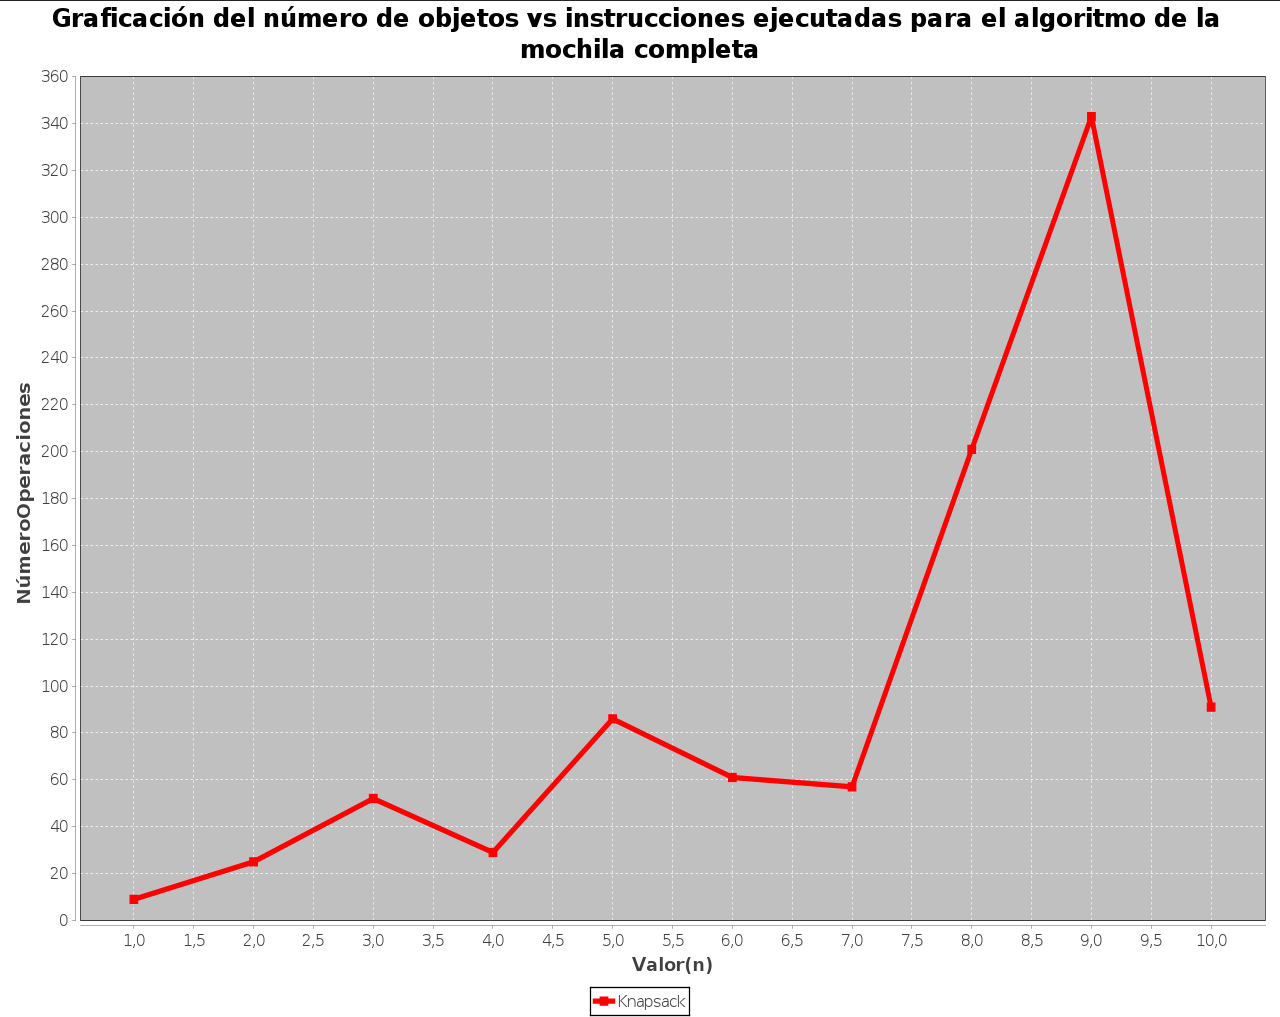
\includegraphics[width=15cm]{Knapsack/GraficaKnapsack1.png}
            \caption{Grafica obtenida de 10 problemas diferentes de la mochila entera con el número de objetos ascendentemente y un peso máximo de la mochila arbitrario para cada configuración}
            \label{GraficaKnapsack1}
        \end{figure}
        
        Se observa en la figura \ref{GraficaKnapsack1} una curva irregular que no nos aporta indicio alguno de la complejidad del algoritmo. Así pues intentamos mantener el orden ascendente del número de objetos pero consideraremos el valor de \textbf{P} igual a 10 en todas las configuraciones(figura \ref{GraficaKnapsack2} ):
        
        \begin{figure}[h!]
            \centering
            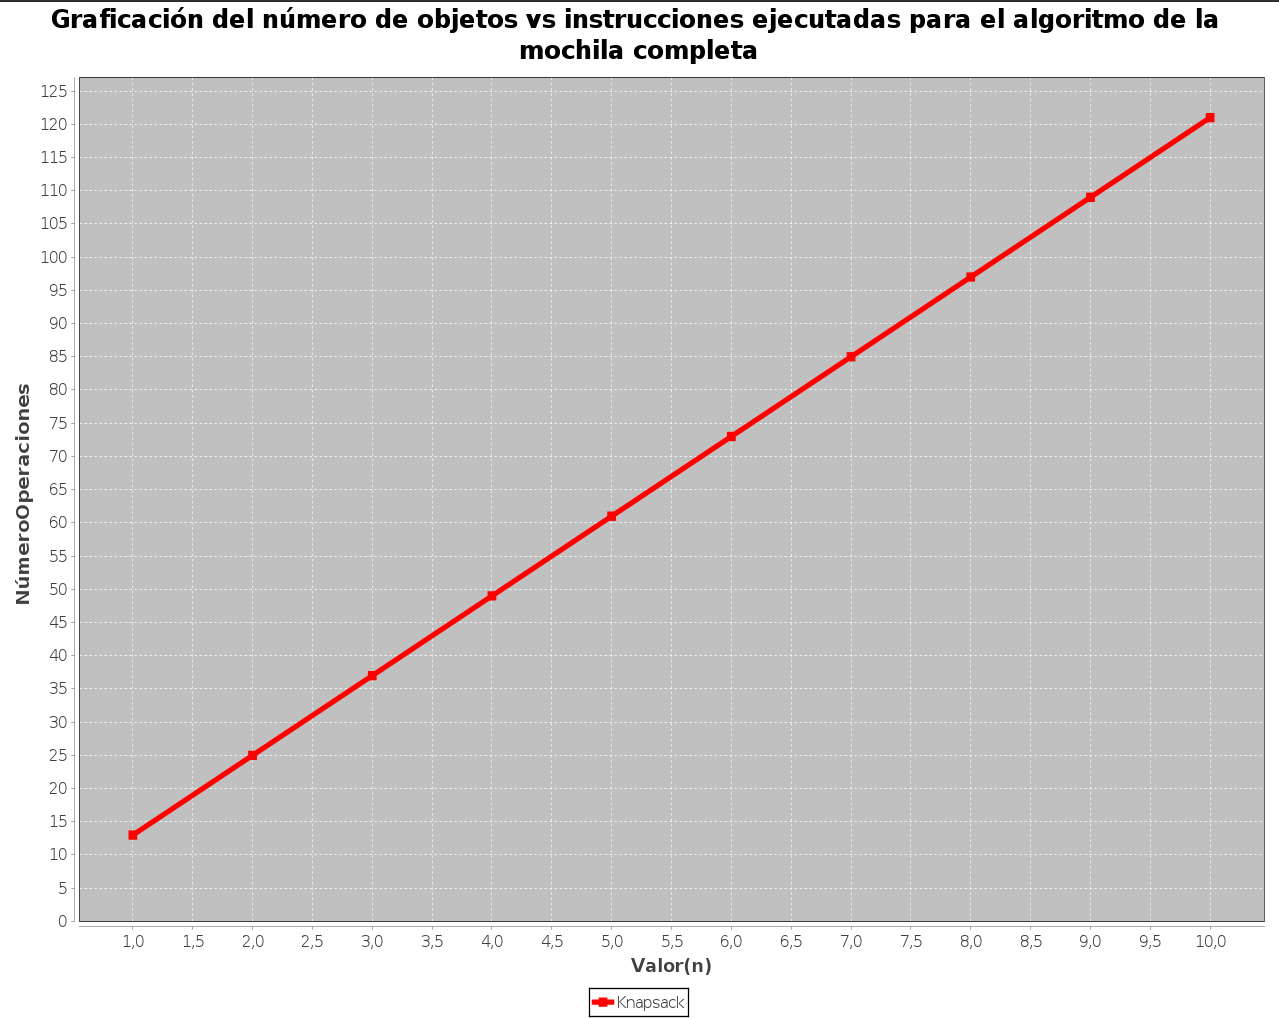
\includegraphics[width=15cm]{Knapsack/GraficaKnapsack2.png}
            \caption{Gráfica generada de 10 problemas diferentes para la mochila entera con un tamaño máximo para todas las mochilas igual}
            \label{GraficaKnapsack2}
        \end{figure}
        
        Y curiosamente para este tipo de configuración en la figura \ref{GraficaKnapsack2} se muestra una complejidad lineal, con una recta que se encuentra desplazada en el eje de las ordenadas, lo que nos sugeriría que existe o existen términos que multiplican a la \textbf{n} y/o que se suman como constante a la \textbf{n}, pudiendo ser el valor de \textbf{P} uno de estos términos.\\
        
        Por último para confirmar esta hipótesis se opta por asignar a cada configuración de mochilas $n=P$, generando la siguiente gráfica en la figura \ref{GraficaKnapsack3}:\\
        \begin{figure}[h!]
            \centering
            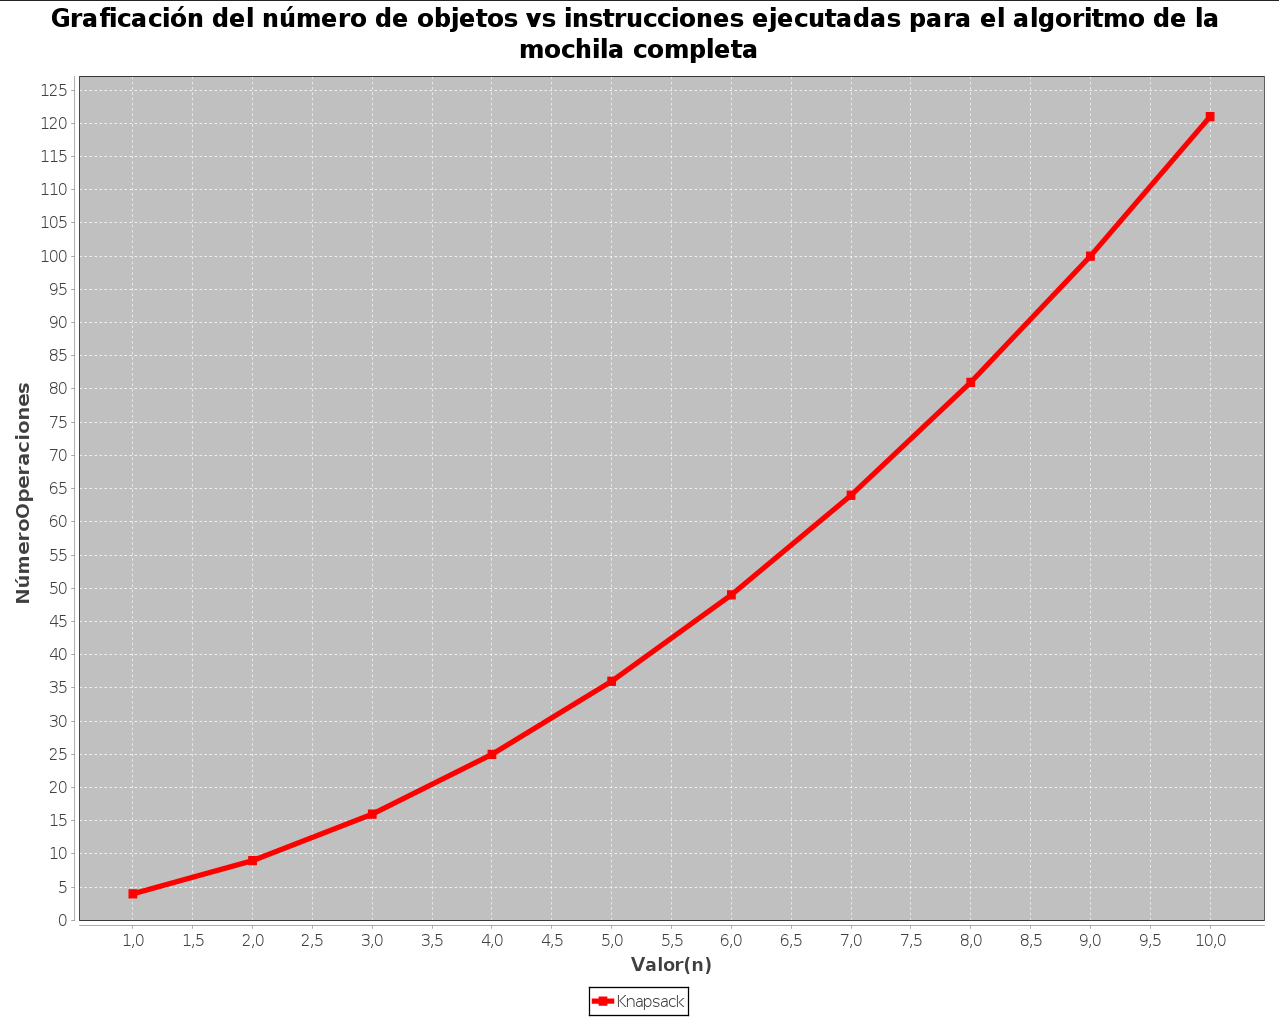
\includegraphics[width=15cm]{Knapsack/GraficaKnapsack3.png}
            \caption{Grafica obtenida para 10 problemas diferentes de la mochila entera donde el número de objetos es igual al peso máximo de la mochila \textbf{P}}
            \label{GraficaKnapsack3}
        \end{figure}
        La curva observada en la figura \ref{GraficaKnapsack3} nos confirma que el término \textbf{P} forma parte de un producto con el número de objetos seleccionables para obtener el comportamiento cuadrático mostrado, explicando así el desplazamiento de la curva en el eje de las ordenadas para la figura \ref{GraficaKnapsack2}, aunque siendo más estrictos para los puntos obtenidos es necesario agregar una constante que debe de pertenecer a las operaciones de asignación, entre otras, que utiliza el algoritmo.\\
        
        Con estas tres gráficas(\ref{GraficaKnapsack1},\ref{GraficaKnapsack2},\ref{GraficaKnapsack3}) afirmamos entonces que la complejidad del algoritmo para la mochila entera se encuentra en función del producto de \textbf{n} y \textbf{P}, quedándonos entonces:
        \begin{equation*}
            K(n,P) \in \Theta(n*P)
        \end{equation*}

\newpage

\section*{Función test}
    El método \textbf{test} funciona como un algoritmo de \textit{Backtracking}, de forma que va construyendo la solución a través de restricciones. Es necesaria esta función pues la construcción de la tabla nos va a asegurar el beneficio máximo para un peso máximo, pero no nos indica con que objetos construye este beneficio, cumpliendo esta necesidad el método \textbf{test}.\\
    
    Inicia su recorrido en la casilla para el beneficio máximo encontrado(celda en la última columna y última fila), y se desarrolla como una función espejo a la de la construcción de la misma tabla.\\
    
    Verifica si la celda en la misma columna pero de la fila anterior tiene un valor diferente, si no fuera el caso significaría que cuando se construyó la tabla, la solución óptima que no consideraba al objeto de la celda actual nos otorga un beneficio mayor a que se considerara este objeto, por lo tanto el valor de la fila anterior solamente es copiado en la fila actual; Esto implicaría en el método que se analiza que no fue construida la solución con este objeto y únicamente se realiza la siguiente iteración con la disminución en la unidad de la fila en la que se analiza la celda.\\
    
    En el caso contrario, donde el valor de la celda actual y el de la celda en la fila anterior sean diferentes, implica que en la elaboración de la tabla la consideración del beneficio del objeto actual nos otorga una solución mayor al de la obtenida para el mismo peso pero considerando unicamente los objetos anteriores;Esto permite considerar al método que el objeto correspondiente a esta fila participa en la suma para la obtención del beneficio máximo. Después entonces se agrega el objeto a los ingresados en la mochila, índice de las columnas disminuye tanto como el valor del peso del objeto correspondiente a la fila y se disminuye en la unidad el índice de la fila.\\
    
    Se itera esta condición hasta llegar a la primer celda, la cual siempre tendrá el valor 0, y es aquí cuando el algoritmo puede terminar su ejecución.\\
    
    La implementación de este algoritmo fue modificado para operar iterativamente, a diferencia del mostrado en el video de clase donde funciona de forma recursiva. El pseudocódigo entonces se muestra en la figura \ref{PseudocodigoTest}
    
    \begin{figure}[h!]
        \centering
        \begin{verbatim}
            Entrada:w
            Salida:m(Lista con los índices de los objetos que se deben ingresar en la mochila)
            
            fila=n+1
            columna=P+1
            while fila > 0 and columna > 0 do
                if g[fila,columna] != g[fila-1,columna]
                    m.push(fila-1)
                    columna = columna - w[fila-1]
                fila --
        \end{verbatim}
        \caption{Pseudocódigo de la implementación recursiva para el algoritmo \textbf{test}}
        \label{PseudocodigoTest}
    \end{figure}
    
    \subsection*{Pruebas funcionamiento}
        Para mostrar los resultados obtenidos de la función \textbf{test}, se van a considerar 2 problemas para la mochila entera:\\
        
        \textbf{Mochila con 5 objetos}\\
        
            Definimos una mochila con el peso máximo de \textbf{15} y la cual debemos de llenar con el máximo beneficio posible con 5 objetos dados(figura \ref{MochilaObjetos5}):
            
            \begin{figure}[h!]
                \centering
                    \begin{itemize}
                        \item Objeto 1 : w=12, b=4
                        \item Objeto 2 : w=2, b=2
                        \item Objeto 3 : w=1, b=1
                        \item Objeto 4 : w=4, b=10
                        \item Objeto 5 : w=1, b=2 
                    \end{itemize}
                \caption{Pesos y beneficio de cada uno de los 5 objetos seleccionables}
                \label{MochilaObjetos5}
            \end{figure}
            
            Se ingresan estos valores para que el algoritmo encuentre el beneficio máximo. A continuación en la figura \ref{ResultadosMochilaObjetos5} se muestrán los resultados del algoritmo:
            \begin{figure}[h!]
                \centering
                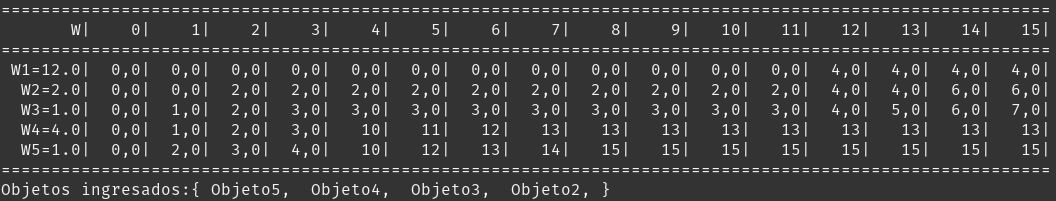
\includegraphics[width=\textwidth]{Knapsack/MochilaObjetos5.png}
                \caption{Resltados obtenidos: Tabla dinámica y el nombre de los elementos que deben de ser ingresados en la mochila para obtener el mayor beneficio}
                \label{ResultadosMochilaObjetos5}
            \end{figure}
            
            Según la última celda de la tabla dinámica, el beneficio máximo que podemos obtener es de \textbf{15}, y según el resultado del método \textbf{test} los objetos que nos otorgan este beneficio son los \textit{Objeto5,Objeto4,Objeto3} y el \textit{Objeto2}.\\
            
            Se realizamos la suma de los beneficios otorgados por estos objetos tenemos:
            $$ 2+1+10+2 = 15$$
            Concordando los resultados obtenidos por el método \textbf{test} con el beneficio máximo obtenible.
        
        \hfill \break
        \hfill \break
        
        \textbf{Mochila con 6 objetos}\\
        
            Ahora definimos una mochila con el peso máximo de \textbf{8} y esta mochila la debemos de llenar con el máximo beneficio posible con 6 objetos dados(figura \ref{MochilaObjetos6}):
            
            \begin{figure}[h!]
                \centering
                    \begin{itemize}
                        \item A : w=1, b=2
                        \item B : w=2, b=5
                        \item C : w=4, b=6
                        \item D : w=5, b=10
                        \item E : w=7, b=13 
                        \item F : w=9, b=16 
                    \end{itemize}
                \caption{Pesos y beneficio de cada uno de los 6 objetos seleccionables}
                \label{MochilaObjetos6}
            \end{figure}
            
            Se ingresan estos valores para que el algoritmo encuentre el beneficio máximo. A continuación en la figura \ref{ResultadosMochilaObjetos6} se muestrán los resultados del algoritmo:
            \begin{figure}[h!]
                \centering
                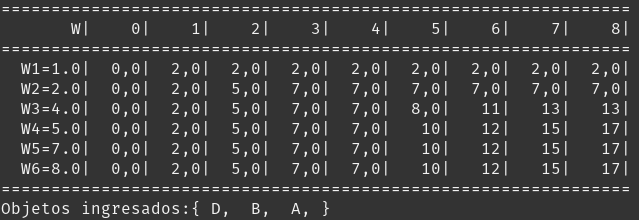
\includegraphics[width=\textwidth]{Knapsack/MochilaObjetos6.png}
                \caption{Resltados obtenidos: Tabla dinámica y el nombre de los elementos que deben de ser ingresados en la mochila para obtener el mayor beneficio}
                \label{ResultadosMochilaObjetos5}
            \end{figure}
            
            Según la última celda de la tabla dinámica, el beneficio máximo que podemos obtener es de \textbf{17}, y según el resultado del método \textbf{test} los objetos que nos otorgan este beneficio son \textit{D,B} y el objeto \textit{A}.\\
            
            Se realizamos la suma de los beneficios otorgados por estos objetos tenemos:
            $$ 10+5+2 = 17$$
            Concordando los resultados obtenidos por el método \textbf{test} con el beneficio máximo obtenible.
        
            
        
\chapter*{Conclusiones}
    \begin{tabular}{l l}
        \multirow{3}{*}{
\includegraphics[width=1.5cm]{Imagenes/imanol.jpg}} &  \\
        & \textbf{Rivero Ronquillo Omar Imanol}\\
        & \\
    \end{tabular}
    \vspace*{3\baselineskip}\\
    Nunca había pensado en las formas en las que se podría optimizar la solución a un problema por medio de un algoritmo programable. Me pareció un enfoque increíble y ahora me parece que tengo claro porque se usan estos algorimos y en qué problemas se les podría dar un uso. A pesar de que en comparación con las prácticas anteriores se tuvieron que incluir más cosas además de los algorimos, para poder probarlos y estudiarlos, me parecieron un gran complemento en mi formación académica.
    
    En conclusión, me gustaría conocer más algoritmos de este tipo, me interesaron especialmente los algoritmos de compresión, aunque puedo estar bastante seguro de que las compresiones modernas deberán de tener una complejidad mayor de aprenderse y comprender su funcionamiento, que seguramente justificaran todo esto con las tasas de compresiones que puedan lograr.
    \\\\
    \begin{tabular}{l l}
        \multirow{3}{*}{
\includegraphics[width=1.5cm]{Imagenes/lalo.jpg}}  &  \\
        & \textbf{Valle Mart\'inez Luis Eduardo} \\
        & \\
    \end{tabular}
    \vspace*{3\baselineskip}\\
    
    
\begin{thebibliography}{}

    \bibitem{clase}Luna,B.[Preparación Estudiantil de 10].(2020, Agosto, 22). Sucesión de Fibonacci mediante Programación Dinámica[Archivo de video]. Recuperado de https://www.youtube.com/watch?v=fXCMZ8ilSA8
    
    \bibitem{clasePD}Luna,B.[Benjamín Luna].(2020, Agosto, 22). \textit{Problema de la Mochila Entera con Programación Dinámica}[Archivo de video]. Recuperado de https://www.youtube.com/watch?v=9srgDGnyZKA
    
    \bibitem{articulo1}Ghose T.,(2018, Octubre, 24). What is the Fibonacci Sequence?. Live Science. Recuperado de https://www.livescience.com/37470-fibonacci-sequence.html
    
    \bibitem{MKPV} \textsc{Laabadi, S., Naimi,M., El Amri, H. and Achchab, B.} (2018) \textit{The 0/1 Multidimensional Knapsack Problem and Its Variants: A Survey of Practical}
    
    \bibitem{TP}\textsc{Tutorials Point} \textit{DDA - Dynamic Programming} web:https://www.tutorialspoint.com/design\_and\_analysis\_of\_algorithms/design\_and\_analysis\_of\_algorithms\_dynamic\_programming.htm
    
    \bibitem{W}\textsc{Wikipedia} \textit{Dynamic Programming} web:https://www.tutorialspoint.com/design\_and\_analysis\_of\_algorithms/design\_and\_analysis\_of\_algorithms\_dynamic\_programming.htm
\end{thebibliography}

\end{document}
